\documentclass[a4paper,12pt]{article}

% --- パッケージ ---
\usepackage{amsmath,amssymb}    % 数式用
\usepackage{fancybox}           % 囲み枠
\usepackage{geometry}           % 余白調整
\usepackage{tikz}               % TikZ図
\usetikzlibrary{decorations.pathmorphing,patterns} % バネ・壁の模様

\geometry{margin=25mm}          % 余白設定

% --- 日本語設定(LuaLaTeX用)---
\usepackage{luatexja}
\usepackage{luatexja-fontspec}
\setmainjfont{IPAexMincho}      % 日本語フォント(朝体)

\begin{document}

% ========= 【29】 ========= 済
[29]
\begin{center}
    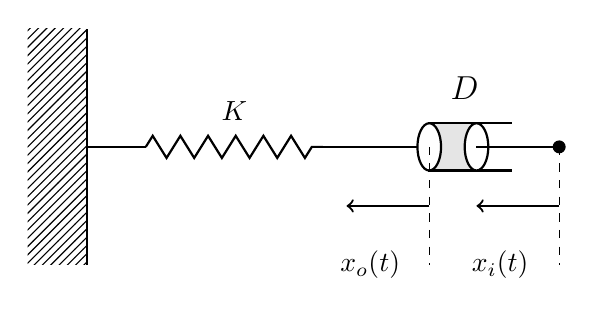
\begin{tikzpicture}[scale=1.5]
      % 固定壁
      \fill[pattern=north east lines] (-0.5,0) rectangle (0,2);
      \draw[thick] (0,0) -- (0,2);
    
      % バネ
      \draw[thick] (0,1) -- (0.5,1);
      \draw[thick, decorate, decoration={zigzag, segment length=10, amplitude=4}] (0.5,1) -- (2,1);
      \node at (1.25,1.3) {$K$};
    
      % --- ダンパー(シリンダー形) ---
\draw[thick] (2,1) -- (2.9,1); % 棒(変更なし)
\draw[thick, fill=gray!20] (2.9,0.8) rectangle (3.3,1.2); % 筒の側面
\draw[thick] (3.3,1.2) -- (3.6,1.2);% 筒の側面(上)
\draw[thick] (3.3,0.8) -- (3.6,0.8);% 筒の側面(下)
\draw[thick, fill=white] (2.9,1) ellipse (0.1 and 0.2);   % 左側の端面(楕円)
\draw[thick, fill=white] (3.3,1) ellipse (0.1 and 0.2);   % 右側の端面(楕円)
\draw[thick] (3.3,1) -- (4.0,1); % ピストン棒 → 始点を 3.5 → 3.3 に変更
\node at (3.2,1.5) {\large $D$};


      % 入力矢印
      \draw[->, thick] (4,0.5) -- (3.3,0.5);
      \node at (3.5,0) {$x_i(t)$};
    
      % 出力矢印
      \draw[->, thick] (2.9,0.5) -- (2.2,0.5);
      \node at (2.4,0) {$x_o(t)$};
    
      % 支点
      \draw[fill] (4,1) circle (0.05);
    
      % 点線
      \draw[dashed] (2.9,1) -- (2.9,0);
      \draw[dashed] (4.0,1) -- (4.0,0);
    \end{tikzpicture}
    \end{center}

% ========= 【30】 ========= 済
[30]
\begin{center}
    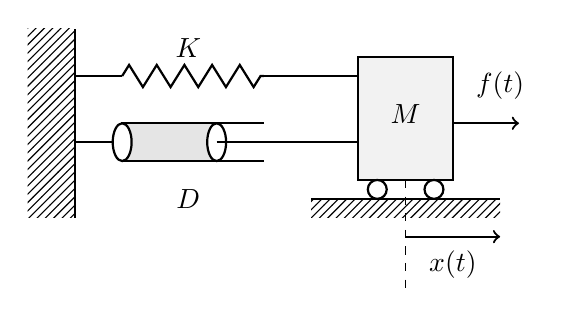
\begin{tikzpicture}[scale=1.2]
      % 固定壁
      \fill[pattern=north east lines] (-0.5,0) rectangle (0,2);
      \draw[thick] (0,0) -- (0,2);
    
      % バネ
      \draw[thick] (0,1.5) -- (0.5,1.5);
      \draw[thick, decorate, decoration={zigzag, segment length=10, amplitude=4}] (0.5,1.5) -- (2,1.5);
      \draw[thick] (2,1.5) -- (3.5,1.5);
      \node at (1.2,1.8) {$K$};
    
      % ダンパー(シリンダー形式)
      \draw[thick] (0,0.8) -- (0.5,0.8); % 棒
      \draw[thick, fill=gray!20] (0.5,0.6) rectangle (1.5,1.0); % 筒の側面
      \draw[thick] (1.5,1.0) -- (2,1.0); % 筒の上
      \draw[thick] (1.5,0.6) -- (2,0.6); % 筒の下
      \draw[thick, fill=white] (0.5,0.8) ellipse (0.1 and 0.2); % 左端面
      \draw[thick, fill=white] (1.5,0.8) ellipse (0.1 and 0.2); % 右端面
      \draw[thick] (1.5,0.8) -- (3,0.8); % ピストン棒
      \node at (1.2,0.2) {$D$};
    
      % 質量M
      \draw[thick, fill=gray!10] (3,0.4) rectangle (4,1.7);
      \node at (3.5,1.1) {$M$};
      % ローラー追加
        \draw[thick] (3.2,0.3) circle (0.1);
        \draw[thick] (3.8,0.3) circle (0.1);

    
      % 床
      \draw[thick] (2.5,0.2) -- (4.5,0.2);
      \fill[pattern=north east lines] (2.5,0) rectangle (4.5,0.2);
    
      % 座標
      \draw[->, thick] (3.5,-0.2) -- (4.5,-0.2);
      \node at (4,-0.5) {$x(t)$};
      \draw[dashed] (3.5,0.4) -- (3.5,-0.8);
    
      % 外力
      \draw[->, thick] (4,1) -- (4.7,1);
      \node at (4.5,1.4) {$f(t)$};
    \end{tikzpicture}
    \end{center}
    
% ========= 【31】 ========= 済
[31]
\begin{center}
    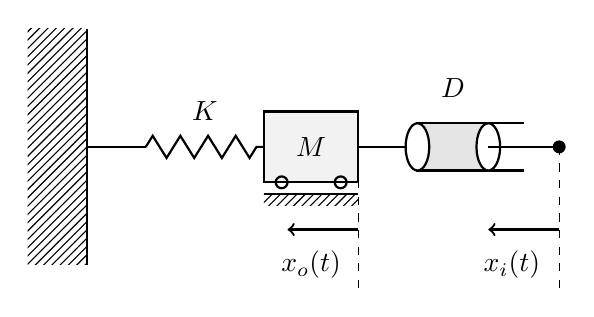
\begin{tikzpicture}[scale=1.5]
      % 固定壁
      \fill[pattern=north east lines] (-0.5,0) rectangle (0,2);
      \draw[thick] (0,0) -- (0,2);

      % バネ
      \draw[thick] (0,1) -- (0.5,1);
      \draw[thick, decorate, decoration={zigzag, segment length=10, amplitude=4}] (0.5,1) -- (1.5,1);
      \node at (1,1.3) {$K$};
    
      % 質量M
      \draw[thick, fill=gray!10] (1.5,0.7) rectangle (2.3,1.3);
      \node at (1.9,1) {$M$};
      % ローラー
      \draw[thick] (1.65,0.7) circle (0.05);
      \draw[thick] (2.15,0.7) circle (0.05);
      % 地面
      \draw[thick] (1.5,0.6) -- (2.3,0.6);
      \fill[pattern=north east lines] (1.5,0.5) rectangle (2.3,0.6);
    
      % ダンパー
      \draw[thick] (2.3,1) -- (2.8,1); % 棒
      \draw[thick, fill=gray!20] (2.8,0.8) rectangle (3.4,1.2); % 筒
      \draw[thick] (3.4,1.2) -- (3.7,1.2); % 筒上
      \draw[thick] (3.4,0.8) -- (3.7,0.8); % 筒下
      \draw[thick, fill=white] (2.8,1) ellipse (0.1 and 0.2);
      \draw[thick, fill=white] (3.4,1) ellipse (0.1 and 0.2);
      \draw[thick] (3.4,1) -- (4,1); % ピストン棒
      \node at (3.1,1.5) {$D$};
    
      % 入力矢印
      \draw[->, thick] (4,0.3) -- (3.4,0.3);
      \node at (3.6,0) {$x_i(t)$};
    
      % 出力矢印
      \draw[->, thick] (2.3,0.3) -- (1.7,0.3);
      \node at (1.9,0) {$x_o(t)$};
    
      % 支点
      \draw[fill] (4,1) circle (0.05);
    
      % 点線
      \draw[dashed] (2.3,1) -- (2.3,-0.2);
      \draw[dashed] (4,1) -- (4,-0.2);
    \end{tikzpicture}
    \end{center}
    
% ========= 【32】 ========= 済
[32]
\begin{center}
  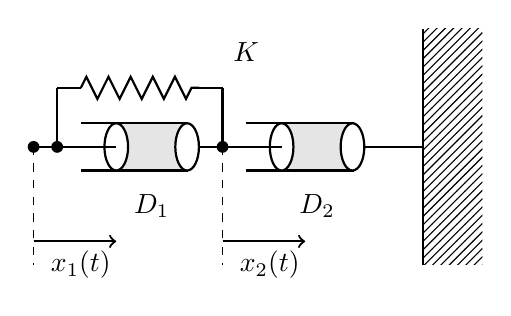
\begin{tikzpicture}[scale=1.5]
    % 固定壁
    \fill[pattern=north east lines] (4,0) rectangle (4.5,2);
    \draw[thick] (4,2) -- (4,0);
  
    % ダンパ D2
    \draw[thick, fill=gray!20] (2.8,0.8) rectangle (3.4,1.2);
    \draw[thick] (2.8,1.2) -- (2.5,1.2);
    \draw[thick] (2.8,0.8) -- (2.5,0.8);
    \draw[thick, fill=white] (2.8,1) ellipse (0.1 and 0.2);
    \draw[thick, fill=white] (3.4,1) ellipse (0.1 and 0.2);
    \draw[thick] (2,1) -- (2.8,1);
    \draw[thick] (3.5,1) -- (4,1);
    \node at (3.1,0.5) {$D_2$};
  
    % ダンパ D1
    \draw[thick, fill=gray!20] (1.4,0.8) rectangle (2.0,1.2);
    \draw[thick] (1.4,1.2) -- (1.1,1.2);
    \draw[thick] (1.4,0.8) -- (1.1,0.8);
    \draw[thick, fill=white] (1.4,1) ellipse (0.1 and 0.2);
    \draw[thick, fill=white] (2.0,1) ellipse (0.1 and 0.2);
    \draw[thick] (0.7,1) -- (1.4,1);
    \node at (1.7,0.5) {$D_1$};
  
    % バネ K
    \draw[thick] (0.9,1) -- (0.9,1.5);
    \draw[thick] (0.9,1.5) -- (1.1,1.5);
    \draw[thick, decorate, decoration={zigzag, segment length=8, amplitude=4}] (1.1,1.5) -- (2.1,1.5);
    \draw[thick] (2.1,1.5) -- (2.3,1.5);
    \draw[thick] (2.3,1) -- (2.3,1.5);
    \node at (2.5,1.8) {$K$};
  
    % 接点
    \fill (0.7,1) circle (0.05);
    \fill (0.9,1) circle (0.05);
    \fill (2.3,1) circle (0.05);

  
    % 点線(基準線)
    \draw[dashed] (0.7,1) -- (0.7,0);
    \draw[dashed] (2.3,1) -- (2.3,0);
  
    % 入力 x₁(t)
    \draw[->, thick] (0.7,0.2) -- (1.4,0.2);
    \node at (1.1,0) {$x_{1}(t)$};
  
    % 出力 x₂(t)
    \draw[->, thick] (2.3,0.2) -- (3,0.2);
    \node at (2.7,0) {$x_{2}(t)$};
  \end{tikzpicture}
  
    \end{center}

% ========= 【33】 ========= 済
[33]
\begin{center}
    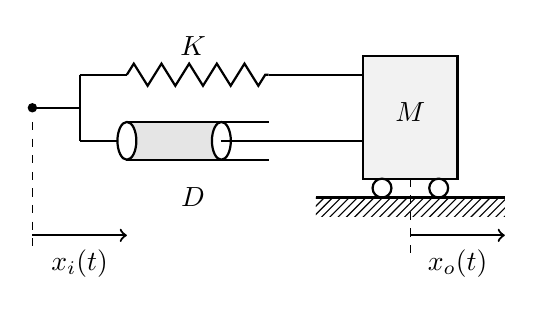
\begin{tikzpicture}[scale=1.2]
      % バネ
      \draw[thick] (0,1.5) -- (0.5,1.5);
      \draw[thick, decorate, decoration={zigzag, segment length=10, amplitude=4}] (0.5,1.5) -- (2,1.5);
      \draw[thick] (2,1.5) -- (3.5,1.5);
      \node at (1.2,1.8) {$K$};
    
      % ダンパー(シリンダー形式)
      \draw[thick] (0,0.8) -- (0.5,0.8); % 棒
      \draw[thick, fill=gray!20] (0.5,0.6) rectangle (1.5,1.0); % 筒の側面
      \draw[thick] (1.5,1.0) -- (2,1.0); % 筒の上
      \draw[thick] (1.5,0.6) -- (2,0.6); % 筒の下
      \draw[thick, fill=white] (0.5,0.8) ellipse (0.1 and 0.2); % 左端面
      \draw[thick, fill=white] (1.5,0.8) ellipse (0.1 and 0.2); % 右端面
      \draw[thick] (1.5,0.8) -- (3,0.8); % ピストン棒
      \node at (1.2,0.2) {$D$};
    
      % 質量M
      \draw[thick, fill=gray!10] (3,0.4) rectangle (4,1.7);
      \node at (3.5,1.1) {$M$};
      % ローラー追加
        \draw[thick] (3.2,0.3) circle (0.1);
        \draw[thick] (3.8,0.3) circle (0.1);

      % 床
      \draw[thick] (2.5,0.2) -- (4.5,0.2);
      \fill[pattern=north east lines] (2.5,0) rectangle (4.5,0.2);
    
      % 座標
      \draw[->, thick] (3.5,-0.2) -- (4.5,-0.2);
      \node at (4,-0.5) {$x_o(t)$};
      \draw[dashed] (3.5,0.4) -- (3.5,-0.4);

      \draw[->, thick] (-0.5,-0.2) -- (0.5,-0.2);
      \node at (0,-0.5) {$x_i(t)$};
      \draw[dashed] (-0.5,1) -- (-0.5,-0.4);

      \draw[thick] (0,0.8) -- (0,1.5);
      \draw[thick] (0,1.15) -- (-0.5,1.15);

      \fill (-0.5,1.15) circle (0.05);

    \end{tikzpicture}
    \end{center}

\newpage
% ========= 【34】 ========= 済
[34]
\begin{center}
    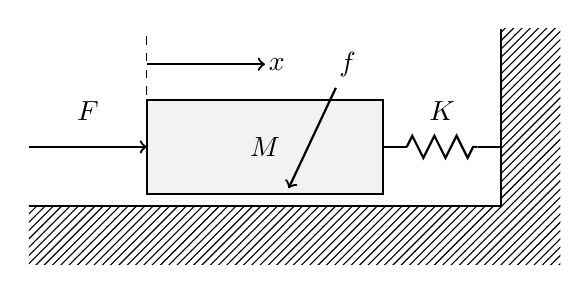
\begin{tikzpicture}[scale=1.5]
      % 固定壁
      \draw[thick] (4,2) -- (4,0.5);
      \fill[pattern=north east lines] (4,0) rectangle (4.5,2);
    
      % バネ
      \draw[thick] (3,1) -- (3.2,1);
      \draw[thick, decorate, decoration={zigzag, segment length=8, amplitude=4}] (3.2,1) -- (3.8,1);
      \draw[thick] (3.8,1) -- (4,1);
      \node at (3.5,1.3) {$K$};
    
      % 質量M
      \draw[thick, fill=gray!10] (1,0.6) rectangle (3,1.4);
      \node at (2,1) {$M$};

      %粘性抵抗係数
      \draw[->, thick] (2.6,1.5) -- (2.2,0.65);
      \node at (2.7,1.7) {$f$};

      % 地面
      \draw[thick] (0,0.5) -- (4,0.5);
      \fill[pattern=north east lines] (0,0) rectangle (4,0.5);
    
      % 外力
      \draw[->, thick] (0,1) -- (1,1);
      \node at (0.5,1.3) {$F$};
    
      % 点線
      \draw[dashed] (1,0.6) -- (1,2);
    
      % 座標
      \draw[->, thick] (1,1.7) -- (2,1.7);
      \node at (2.1,1.7) {$x$};
    \end{tikzpicture}
    \end{center}
    
% ========= 【35】 ========= 済
[35]
\begin{center}
    \begin{tikzpicture}[scale=1.2]
      % 左側(平衡状態)
      \node at (-2,-1)[scale=0.6] {$質量-ばね-まさつ系(平衡状態)$};

        %壁
        \draw[thick] (-3,0) -- (-3,4);
        \draw[thick] (-3,4) -- (-1,4);
        \draw[thick] (-1,0) -- (-1,4);
        \fill[pattern=north east lines] (-3.5,0) rectangle (-3,4);
        \fill[pattern=north east lines] (-3.5,4) rectangle (-0.5,4.5);
        \fill[pattern=north east lines] (-1,0) rectangle (-0.5,4);


        %ばね
        \draw[thick] (-2,1) -- (-2,2);
        \draw[thick, decorate, decoration={coil, segment length=6}] (-2,2) -- (-2,3);
        \draw[thick] (-2,3) -- (-2,4);
        \node at (-2.3,2.5) {$K$};

        %重り
        \draw[thick, fill=gray!10] (-2.9,0.2) rectangle (-1.1,1);
        \node at (-2,0.6) {$M$};

        %粘性摩擦定数
        \draw[->, thick] (-1.3,0) -- (-1.1,0.6);
        \node at (-1.4,-0.2) {$f$};

        %重り
        \draw[dashed] (-2.9,1.2) rectangle (-1.1,2);

        %座標
        \draw[dashed] (-4.5,4) -- (-3,4);
        \draw[dashed] (-4.5,1) -- (-2.9,1);
        \draw[dashed] (-4,2) -- (-2.9,2);

        \draw[<->,thick] (-3.8,4) -- (-3.8,2);
        \node at (-3.95,3) {$y_0$};
        \draw[<->,thick] (-4.3,4) -- (-4.3,1);
        \node at (-4.45,2.5) {$y_1$};
      
      % 左側(平衡状態)
      \node at (2,-1)[scale=0.6] {$力を加えた場合$};

        %壁
        \draw[thick] (3,0) -- (3,4);
        \draw[thick] (3,4) -- (1,4);
        \draw[thick] (1,0) -- (1,4);
        \fill[pattern=north east lines] (3.5,0) rectangle (3,4);
        \fill[pattern=north east lines] (3.5,4) rectangle (0.5,4.5);
        \fill[pattern=north east lines] (1,0) rectangle (0.5,4);


        %ばね
        \draw[thick] (2,1.3) -- (2,2.2);
        \draw[thick, decorate, decoration={coil, segment length=6}] (2,2.2) -- (2,3.1);
        \draw[thick] (2,3.1) -- (2,4);
        \node at (2.3,2.65) {$K$};

        %重り
        \draw[thick, fill=gray!10] (2.9,0.5) rectangle (1.1,1.3);
        \node at (2,0.9) {$M$};

        %粘性摩擦定数
        \draw[->, thick] (2.7,0) -- (2.9,0.6);
        \node at (2.6,-0.2) {$f$};

        %座標
        \draw[dashed] (0.1,4) -- (1,4);
        \draw[dashed] (0.1,1.3) -- (1.1,1.3);
        \draw[dashed] (2.9,1.3) -- (4,1.3);

        \draw[<->,thick] (0.3,4) -- (0.3,1.3);
        \node at (0,2.65) {$y_1$};

        \draw[->,thick] (3.8,1.3) -- (3.8,0.5);
        \node at (3.8,0.3) {$y$};

        
    
    \end{tikzpicture}
    \end{center}
    
% ========= 【36】 ========= 
[36]
\begin{center}
    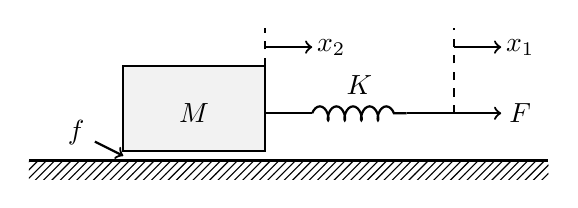
\begin{tikzpicture}[scale=1.2]
      % 地面
      \draw[thick] (-0.5,0) -- (5,0);
      \fill[pattern=north east lines] (-0.5,-0.2) rectangle (5,0);
    
      % 質量M
      \draw[thick, fill=gray!10] (0.5,0.1) rectangle (2,1);
      \node at (1.25,0.5) {$M$};
      \draw[dashed] (2,1.0) -- (2,1.4);
    
      % 摩擦f
      \draw[->,thick] (0.2,0.2) -- (0.5,0.05);
      \node at (0,0.3) {$f$};
    
      % バネ
      \draw[thick] (2,0.5) -- (2.5,0.5);
      \draw[thick, decorate, decoration={coil, segment length=6}] (2.5,0.5) -- (3.5,0.5);
      \node at (3,0.8) {$K$};
      \draw[dashed] (4,0.5) -- (4,1.4);
    
      % 外力
      \draw[->, thick] (3.5,0.5) -- (4.5,0.5);
      \node at (4.7,0.5) {$F$};
    
      % 座標 x2
      \draw[->, thick] (2,1.2) -- (2.5,1.2);
      \node at (2.7,1.2) {$x_2$};
    
      % 座標 x1
      \draw[->, thick] (4,1.2) -- (4.5,1.2);
      \node at (4.7,1.2) {$x_1$};
    \end{tikzpicture}
    \end{center}
    
\end{document}
